%%%%%%%%%%%%%%%%%%%%%%%%%%%%%%%%%%%%
%% PACKAGES
%%%%%%%%%%%%%%%%%%%%%%%%%%%%%%%%%%%%
\documentclass{article}
\usepackage[utf8]{inputenc}
\usepackage[margin=2.0cm]{geometry}
\usepackage{graphicx}
\usepackage{gensymb}
\usepackage{enumerate}
\usepackage{multicol}
\usepackage{amsmath}
\usepackage{hhline}
\usepackage{verbatim}
\makeatletter
\renewcommand*\env@matrix[1][*\c@MaxMatrixCols c]{%
  \hskip -\arraycolsep
  \let\@ifnextchar\new@ifnextchar
  \array{#1}}
\makeatother
\usepackage{mathtools}
\setlength{\skip\footins}{1cm}
\setlength{\parindent}{0pt}
\usepackage{tikz}
\usepackage{fancyvrb}
\usepackage{units}
\usepackage{float}
\begin{document}
\setcounter{MaxMatrixCols}{20}

%%%%%%%%%%%%%%%%%%%%%%%%%%%%%%%%%%%%
%% HEADING
%%%%%%%%%%%%%%%%%%%%%%%%%%%%%%%%%%%%
\rule{\textwidth}{1pt}
Advanced Network Security \hfill Yorick de Boer, 4287304 \\
Project 4 \\
\rule{\textwidth}{1pt}
\vspace{0.5cm}

%%%%%%%%%%%%%%%%%%%%%%%%%%%%%%%%%%%%
%% CONTENTS
%%%%%%%%%%%%%%%%%%%%%%%%%%%%%%%%%%%%
\section{Task 1}
About the algorithm used in IPTables can be concluded that it has a time complexity of $O(N)$.

Instead of 2 million rules a maximum of $20000$ with steps of $1000$ was used because manually adding 2 million rules rules takes ridiculously long. Doing more is possible, but this was enough to come to the conclusion for the used algorithm. (Only later I found out there is a faster way by using the backup option.)

\begin{figure}[H]
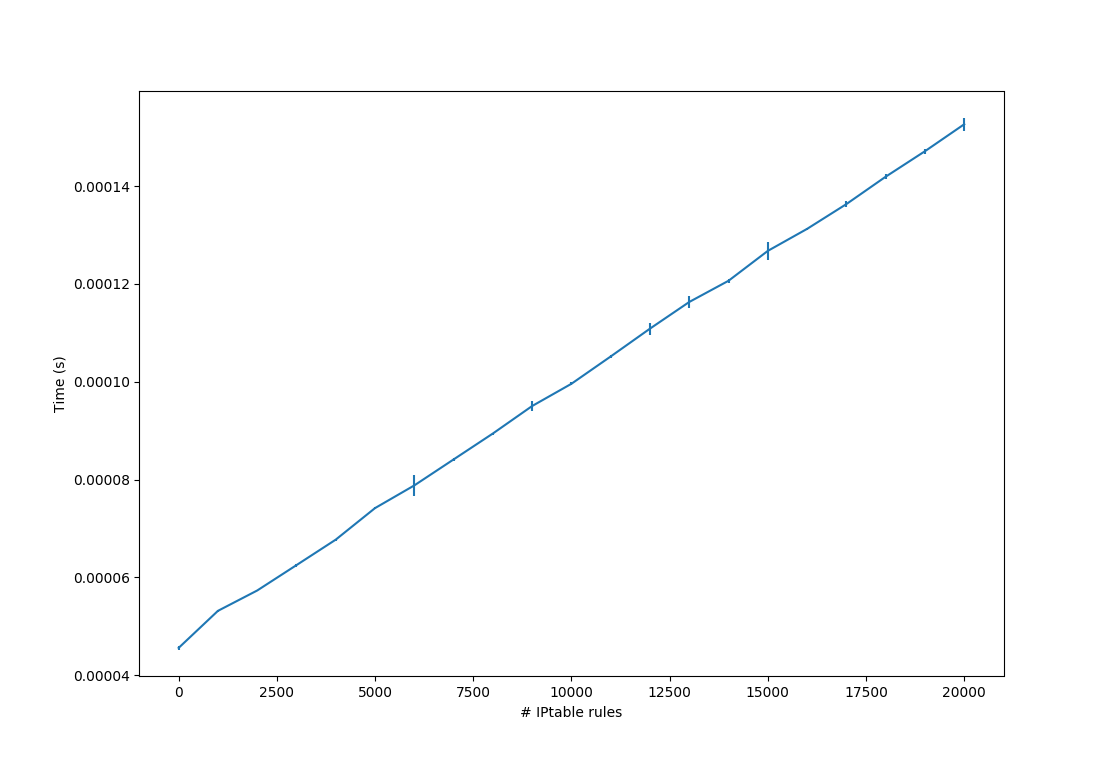
\includegraphics[scale=0.5]{task1}
\end{figure}

\section{Task 2}
A method to restructure the same filtering rules to increase performance, would be to do filter per range. However my current rule set consists of random ips so this is not really an option for me. \\
\\
The internal pattern matching can be made more efficient trough IPSet, because this is a set and a (hash)set has a lookup time of O(1). Again the test was not run over 2 million ips. It may be possible that the set table has a maximum size and starts doing chaining when a collision occurs if I would have been able to test with more rules. The time complexity will increase then.

\begin{figure}[H]
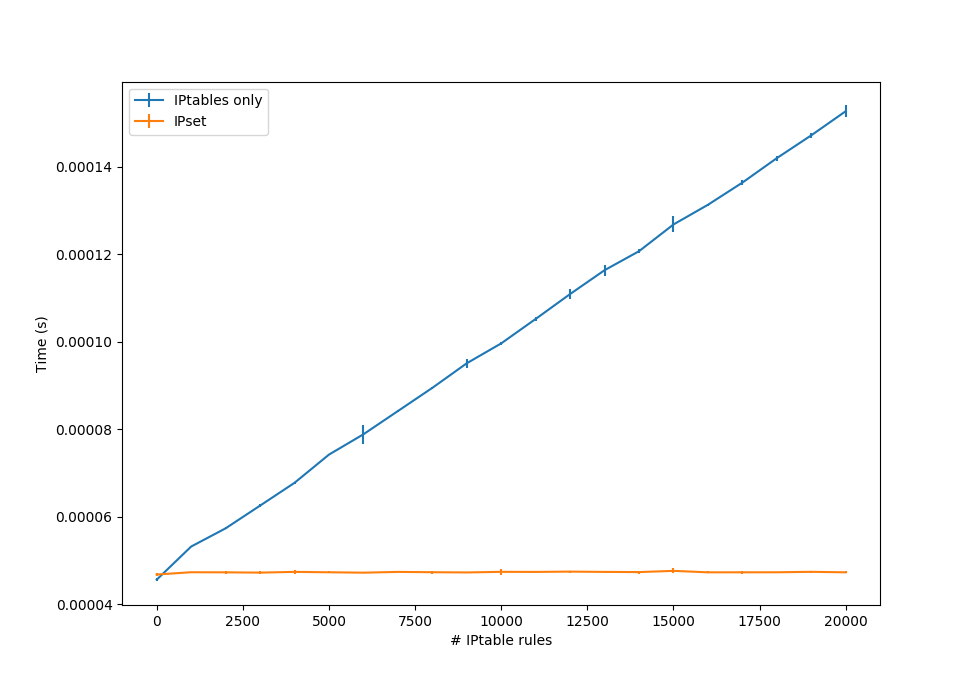
\includegraphics[scale=0.6]{task2}
\end{figure}

\section{Task 3}
(see code: datastructures/bloomfilter.py) \\
For the IPTable datastructure a Python list structure was used. For the hashtable a Python dict structure. The difference between the hashtable and bloom filter is $0.1\cdot10^{-5}$, where the hashtable is the fastest. This difference can probably be ascribed to the difference in implementation and language. For instance the hashtable has a C backend, while the bloom filter is partly Python.
\begin{figure}[H]
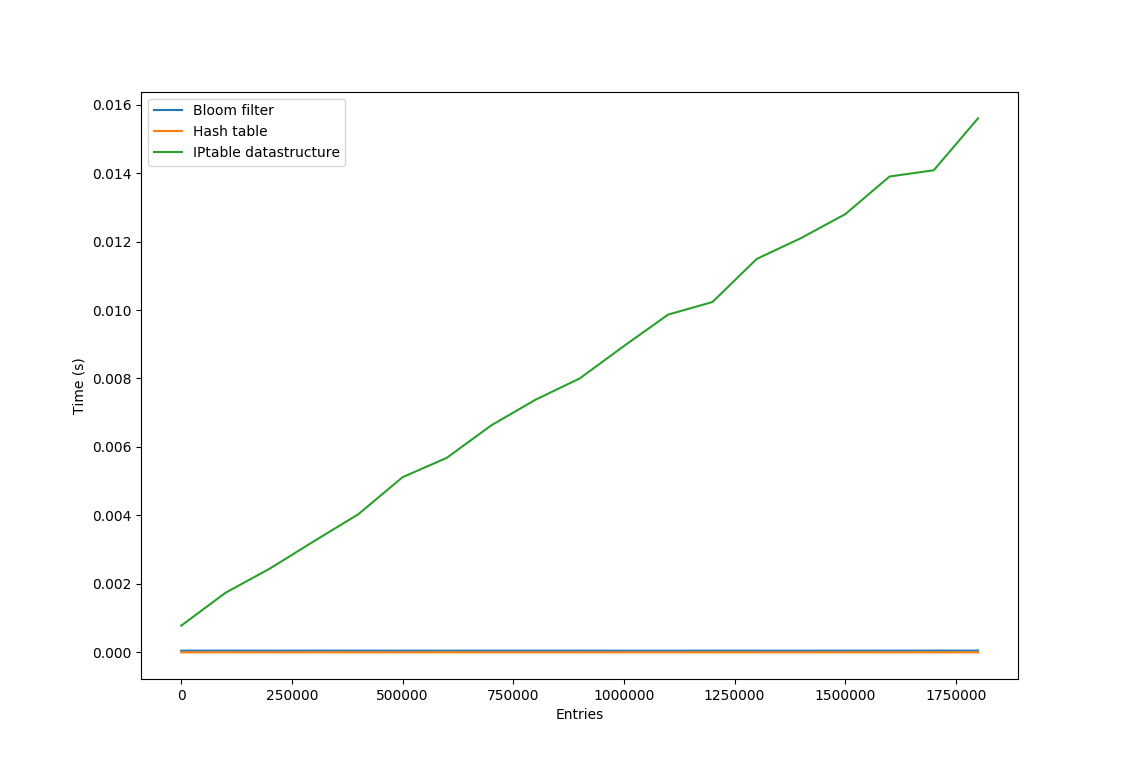
\includegraphics[scale=0.55]{task3}
\end{figure}

\section{Task 4}
(see code: datastructures/trie.py) \\
Theoretically you would expect the execution time to halve between single bit stride an a two bit stride, because half the comparisons have to be done.

\begin{verbatim}
trie 1 bit adjecent 7.025880 seconds
trie 2 bit adjecent 4.624962 seconds
trie 1 bit random 7.507375 seconds
trie 2 bit random 4.756982 seconds
\end{verbatim}

As can be seen from above results the execution time is not exactly halved, but is definitely less between single bit and two bit tries. The difference between the random adjacent addresses is there but is not really significant especially not when the bit length is increased.

\end{document}
